%31.10.2024, lecture 5


\section{Symmetric Encryption}


\begin{definition}
	\emph{Symmetric-key} (Alice and Bob hold the same private key) encryption scheme is secure in multiple-message setting if
	\[
		\text{the same as a single message, but}
	.\] an adversary is given a sequence of messages (generated by $M_S$) encrypted with the same key
	\[
		\text{and andversary is aked to break them all}
	.\] 
\end{definition}
By SKES we denote Symmetric-Key Encryption Scheme.

\subsection{Wrong Construction}

Assume we have some "secret book" which is a PRG and we will use bits from it to encrypt messages.
We have publicly known PRG $G$ and some symmetric key  $\sk$:
 \[
E(\sk, \msg) = \msg \oplus G(\sk) = (b_1 \oplus G_1(\sk)) \circ \ldots \circ (b_p \oplus G_p(\sk))
.\] 
Where $b_i, G_i$ are consequent bits of the message and the PRG, respectively.

An attack:
 \[
	 \msg = E(\sk, 0^{p}) \oplus E(\sk, \msg)
.\] 
So, if we somehow learned $E(\sk, 0^{p})$ we can decrypt anything.
And even worse, one can decrypt it without knowing $E(\sk, 0^{p})$.
Assume two messages $\msg \neq \msg'$, then
\[
\sk_i = (E_i(\sk, \msg) \oplus E_i(\sk, \msg')) \oplus (\msg_i \oplus \msg'_i)
.\] \todo{fix}
\begin{exercise}
	Prove formally that this attack is successful: this system is not semantically secure for multiple messages.
\end{exercise}

\subsection{State-based Stream Cipher}

Assume that we have two participants and that most messages are not lost.
Let $G \colon \{0, 1\}^{n} \to  \{0, 1\}^{n + 1}$ be a PRG.
Choose $s$ from $U_n$ as a permanent key.
We maintain a counter and change the "book" fragment accordingly.

The initial state is $(0, s)$.
The state transition $(i, s') \to (i + 1, G(s')_{1\ldots n})$ (i.e. new seed is a first  $n$ bits of  $G(s')$) updates the state, where the last bit $b_{n + 1} \coloneqq G(s')_{n + 1}$ is used for encryption: $E(b) = b_{n + 1} \oplus b$.

If messages are lost, it takes proportional time to recover $s'$ by repeating $G$.
On the decryption side, if a message is lost (and we are notified of the loss), we must update our state many times, proportional to the number of bits lost, before decoding the next bit.

\begin{exercise}
    Prove that this scheme is secure.
\end{exercise}

\subsection{Pseurodandom Functions}

We will construct an encryption scheme based on pseudorandom functions.
The idea is to use a truly random function as a model and prove that our construction is secure.
We generate $f_{\zeta}$ that appears random and show that it is indistinguishable from a truly random function.

\begin{definition}[Pseudorandom function family, prff]
    A prff is a family of functions $\{f_{\zeta}\}_{\zeta}$, where each $f_{\zeta} \colon \{0, 1\}^{n} \to \{0, 1\}^{n}$ is computed by Boolean circuits generated by a polynomial-time algorithm $Z \colon (1^{n}, r_Z) \to f_{\zeta}$.
    The function $f_{\zeta}$ is indistinguishable from a truly random function.
    For any adversary $A$:
    \[
        \left|\Pr_{A, y}[A(y, 1^{n}) = 1 \mid y \gets f_{\zeta}(U_n)] - \Pr_{A, R, x}[A(x, 1^{n}) = 1 \mid x \gets R(U_n)]\right| < \varepsilon(n),
    \] 
    where $R \colon \{0, 1\}^{n} \to \{0, 1\}^{n}$ has a uniformly random truth table.
\end{definition}

Small $\zeta$ serves as an exponentially large "code book".
\begin{remark}
We use  $\zeta$ and  $f_{\zeta}$ interchangeably.
\end{remark}

\begin{scheme}
	One can construct a prff using $2n$-PRG  $G \colon \{0, 1\}^{n} \to  \{0, 1\}^{2n}$.
	Split $G$'s output into two $n$-bit parts $G(x) = G_0(x) \circ G_1(x)$.
	Then, take $s \gets U_n$ and compute
	\[
		\zeta_s(b_1 b_2 \ldots b_n) = G_{b_n}(G_{b_{n - 1}}(\ldots (G_{b_1}(s)) \ldots))
	.\] 
	\begin{figure}[htpb]
		\centering
		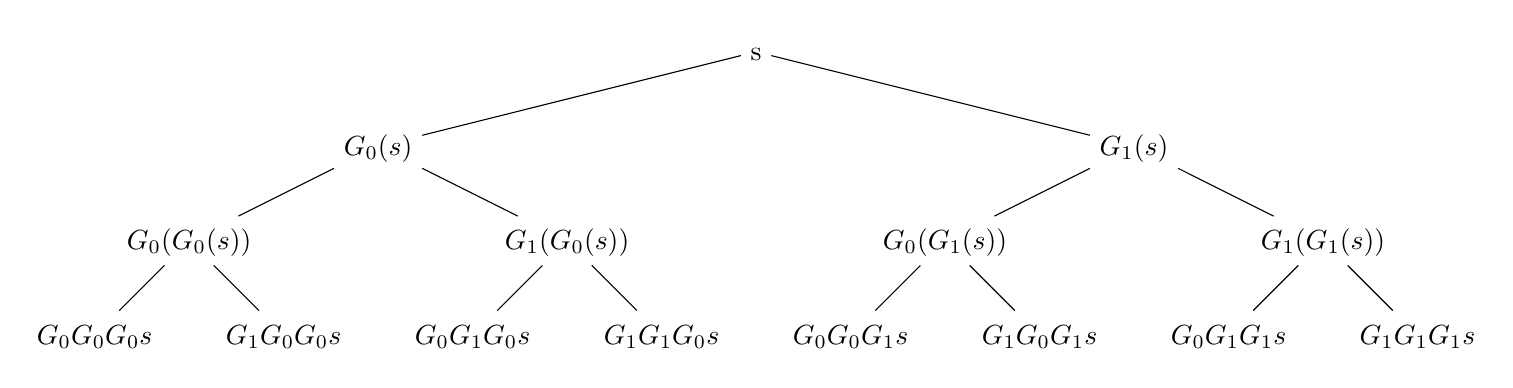
\begin{tikzpicture}[
  level 1/.style={sibling distance=120mm},
  level 2/.style={sibling distance=60mm},
  level 3/.style={sibling distance=30mm},
  every node/.style={text height=2ex, text depth=.5ex},
  scale=0.8
]
  % Root node
  \node {s}
    child {node  {$G_0(s)$}
      child {node  {$G_0(G_0(s))$}
        child {node  {$G_0 G_0 G_0 s$}}
        child {node  {$G_1 G_0 G_0 s$}}
      }
      child {node  {$G_1(G_0(s))$}
        child {node  {$G_0 G_1 G_0 s$}}
        child {node  {$G_1 G_1 G_0 s$}}
      }
    }
    child {node  {$G_1(s)$}
      child {node  {$G_0(G_1(s))$}
        child {node  {$G_0 G_0 G_1 s$}}
        child {node  {$G_1 G_0 G_1 s$}}
      }
      child {node  {$G_1(G_1(s))$}
        child {node  {$G_0 G_1 G_1 s$}}
        child {node  {$G_1 G_1 G_1 s$}}
      }
    };

\end{tikzpicture}
		\caption{Tree of encodings.}
		\label{fig:tree_encodings}
	\end{figure}
	See \Cref{fig:tree_encodings}.
	I.e. each path from root to a leaf is some encoding of a message.
\end{scheme}
\begin{proof}
	If it isn't a prff, hence there is an adversary $D$ that distinguish 
	 \[
		 \zeta_s(b_1 b_2 \ldots b_n) = G_{b_n}(G_{b_{n - 1}}(\ldots (G_{b_1}(s)) \ldots)) \quad \text{from} \quad R(b_1 \ldots b_n)
	.\] 
	Then, we will distinguish $x_1^{l} \circ x_1^{r}, x_2^{l} \circ x_2^{r}, \ldots, x_{p}^{l} \circ x_{p}^{r}$ from truly random source.
	For fixed subtree of our tree, if one substitute random $r$ into it, hence it would give a distribution.
	Using our basic idea, since leaves are distinguishable, hence there is a vertex such that one can distinguish between two its children.
	See \Cref{fig:distinguishable_children}.
		\begin{figure}[htpb]
		\centering
		\begin{tikzpicture}[
  level 1/.style={sibling distance=120mm},
  level 2/.style={sibling distance=60mm},
  level 3/.style={sibling distance=30mm},
  every node/.style={text height=2ex, text depth=.5ex},
  scale=0.8
]
  % Root node
  \node {}
    child {node  {$r_0$}
      child {node  {$G_0(r_0)$}
        child {node  {$G_0 G_0 r_0$}}
        child {node  {$G_1 G_0 r_0$}}
      }
      child {node  {$G_1(r_0)$}
        child {node  {$G_0 G_1 r_0$}}
        child {node  {$G_1 G_1 r_0$}}
      }
    }
    child {node  {$r_1$}
      child {node  {$G_0(r_1)$}
        child {node  {$G_0 G_0 r_1$}}
        child {node  {$G_1 G_0 r_1$}}
      }
      child {node  {$G_1(r_1)$}
        child {node  {$G_0 G_1 r_1$}}
        child {node  {$G_1 G_1 r_1$}}
      }
    };

\end{tikzpicture}
		\caption{Distinguishable children.}
		\label{fig:distinguishable_children}
	\end{figure}
	\todo{finish}

\end{proof}
\begin{remark}
A standard definition says that $Z$ generates an index, and  $f_{\zeta}(x)$ is computed by a polynomial-time algorithm $F(\zeta, x)$.
\end{remark}
\begin{exercise}
	Observe, that this definition is equivalent to the one given above.
\end{exercise}

\subsection{Symmetric-Key Encryption Scheme Based on prff}

\begin{scheme}
\begin{itemize}
	\item To encode an $n$-bit message, define a "proto-scheme":
		 \[
		E(\zeta, \msg, r_E) = (\zeta(r_E) \oplus \msg, r_E)
		,\] 
		where $\zeta \gets Z(1^{n})$ serves as a key and $r_E \gets U$ is our randomness ($r_E$ is independent with $\zeta$).

	\item To encode messages of arbitrary length, cut them into pieces:
		\begin{align*}
			E'(\zeta, \msg, r_E) = (|\msg|, &E(\zeta, \msg[1\ldots n], r_E[1 \ldots n]), \\
										&E(\zeta, \msg[n + 1 \ldots 2n], r_E[n + 1 \ldots 2n]), \ldots)
		.\end{align*}
		It is worth mentioning, that we use the same symmetric key, but different randomness for each piece.
\end{itemize}
\end{scheme}
\begin{lemma}
	This scheme is secure.
\end{lemma}
\begin{proof}
	It is enough to prove that the proto-scheme is secure in multiple-message setting.
	If an adversary distinguishes sequences
	\[
		\{(\zeta(r_i) \oplus \msg^{(i)}, r_i)\}_{i} \quad \text{from} \quad \{(\zeta(r_i') \oplus \underbrace{\rho^{(i)}}_{\text{random}}, r_i')\}_{i} 
	.\] 
	Then, we can distinguish either
	\[
		\zeta \quad \text{and} \quad R
	.\] Where $R$ is a truly random function.
	Or
	\[
		\{(R(r_i) \oplus \msg^{(i)}, r_i)\}_{i} \quad \text{from} \quad \{(R(r_i') \oplus \rho^{(i)}, r_i')\}_{i} 
	.\] 
	But the first one is impossible since $\zeta$ is pseudo random function.
	And the second one is impossible since $R$ is truly random.
\end{proof}


\subsection{Exchanging Keys}

If we have a secure channel, we can simply send the key.

\begin{algorithm}[Diffie-Hellman]
	For a passive adversary, to exchange a key:
	\begin{itemize}
		\item Generate public prime $p \in \mathbb{P}$ and a generator $g \colon Z_{p}^{*} = \{g^{k}\}_{k} $ 
		\item Alice chooses $a$ and sends  $g^{a} \mod p$
		\item Bob chooses $b$ and sends  $g^{b} \mod p$
		\item Now they both have $g^{ab} \equiv_p (g^{a})^{b} \equiv_p (g^{b})^{a}$ (their private keys).
	\end{itemize}
	By assumption that given $h$ it is infasible to check that  $h = g^{ab} \mod p$ from public info.
\end{algorithm}

\subsection{Possible Attacks}

\begin{itemize}
	\item CPA: Chosen Plaintext Attack: adversary can encrypt any messages of their choice.
		Does not add any power to the adversary, since everybody can encrypt anything.
		In private key/symmetric schemes, it adds some power.

	\item CCA: Chosen Ciphertext Attack: adversary can decrypt any ciphertexts of their choice (except target message).
		Adversary gets before (a priori) or after (a posteriori) the ciphertext.
		The prff-base construction is already secure under a-priori CCA, can be made secure under a-posteriori CCA.
		For public-key encryption, additional work is required.
\end{itemize}
